\section{Codifiche e riduzioni}

\subsection{Codifiche ragionevoli}

Ci interessa misurare la complessità di un problema in funzione del tempo e spazio necessari a risolverlo al crescere della dimensione dell'input. \\
Ma lo stesso input puó essere codificato in modi diversi, con dimensioni diverse. \\

\textbf{Esempio:} \\
Se l'input è un grafo $x = (V, E)$ rappresentato tramite liste di adiacenza la dimensione dell'input è $n = |V| + |E|$. \\
Se invece il grafo viene codificato tramite matrice di adiacenza, la dimensione dell'input è $n = |V|^2$. \\
In questo caso non cambia molto, perché $|E| \leq |V|^2$. \\

\textbf{Esempio:} \\
Se l'input é un numero, viene tipicamente codificato in notazione posizionale (di solito binaria, decimale o esadecimale).
La lunghezza della rappresentazione posizionale di un numero richiede una quantità logaritmica di cifre. \\
Di conseguenza, quando l'input $x$ é un numero rappresentato in notazione posizionale, $n = log(x)$. \\
Se invece $x$ fosse rappresentato in unario, allora la lunghezza della sua codifica sarebbe uguale al numero stesso: $n = x$. \\

\textbf{La codifica dell'input puó alterare l'analisi di complessitá.} \\

\textbf{Esempio:} \\
Vogliamo calcolare il fattoriale di un numero naturale $x$. Consideriamo una versione naive che itera su tutti i numeri da 1 a x: $f(n) = f(log(x)) = x$. \\
La soluzione trovata impiega tempo esponenziale su $n$: $f(n) = O(2^n)$. \\
Si potrebbe codificare $x$ in unario: in quel caso avremmo che $x = n$ e il tempo risulterebbe essere una funzione lineare: $f(n) = O(n)$. \\

\textbf{Perché la misura che effettuiamo sia corretta, la codifica dell'input deve essere ragionevole.} \\


\newpage
\subsection{Riduzioni}
Una riduzione traduce un'istanza di un problema in un'istanza di un altro problema. \\
Poi usa la soluzione del secondo problema per risolvere il primo. \\
La traduzione deve essere:
\begin{itemize}
    \item Corretta: la risposta dell'istanza tradotta deve essere la stessa della risposta dell'istanza originale.
    \item Efficiente: la traduzione deve essere eseguita in tempo polinomiale rispetto alla dimensione dell'input originale. \\
    In questo modo, se il secondo problema é risolvibile in tempo polinomiale, anche il primo lo é. \\
\end{itemize}

\subsubsection{Riduzione di $\BIPARTITEMATCHING$ a $\MAXFLOW$}
Sia $G = (U, V, E)$ un grafo bipartito. $U, V$ sono due insiemi di vertici con la stessa cardinalitá $|U| = |V|$. \\ 
Gli archi vanno solo da $U$ a $V$: $E \subseteq U \times V$. \\
Un \textbf{matching} è un insieme di archi $M \subseteq E$ tale che ogni vertice di $U$ ha un arco in $M$ verso uno e un solo vertice di $V$. \\

Per ridurlo a $\MAXFLOW_D$ possiamo trasformare $G$ in un network, 
aggiungendo un nodo $s$ e archi $(s, u)$ per ogni $u \in U$ 
e un nodo $t$ con archi $(v, t)$ per ogni $v \in V$. \\
Settando $c(u, v) = 1$ per ogni arco $(u, v)$, possiamo concludere che
$B$ ha un matching se e solo se la rete ha un flusso di valore $|U|$.

\begin{figure}[h!]
    \centering
    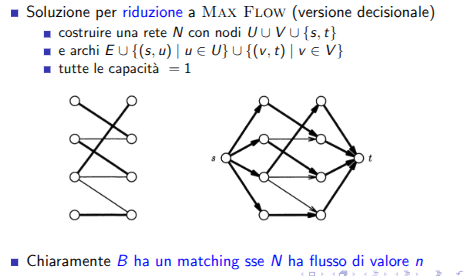
\includegraphics[width=\textwidth]{images/bipartite_matching.png}
\end{figure}